

这本书的的目的是教会大家如何像计算机科学家一样思考。计算机科学用严谨的语言来表明思想,尤其是计算。像工程师,他们设计,把各个组件装配成系统并且在可选方案中评估出折中方案。像科学家,他们研究复杂系统的性能,做出假定并且测试假设。


\index{解决问题}

对一个计算机科学家来说最重要的是解决问题。解决问题意味着清晰明确的阐述问题,积极思考问题答案,并且清楚正确的表达答案的能力。实践证明:学习如何编程是一种很好的机会来练习解决问题的技巧。这也是为什么把这章叫做“编程的方式“。\\

一方面,你将学习编程,一个非常有用的技巧。另一方面你将会把编程作为一种科技。随着我们的深入学习,这点会渐渐明晰。

\section{Python编程语言}
\index{编程语言}
\index{语言!编程}

我们将要学习的编程语言是Python。Python仅是高级语言中的一种,你可能
也听说过其他的高级编程语言,比如C,C++,Perl,和Java。\\

也有一些低级语言,有时也被称为机器语言或者汇编语言。一般来说,计算机
只能执行用低级语言编写的程序。所以,用高级语言编写的程序在执行前必须
做相应的处理。这会花费一定的时间,同时这也是高级语言的“缺点“。\\

\index{移植性}
\index{高级语言}
\index{低级语言}
\index{语言!高级}
\index{语言!低级}

然而,高级语言的优点也是无限的。首先,用高级语言编程是一件非常容易的。
用高级语言编程通常花费的时间比较少,同时编写的程序简短,易读,易纠错
。第二,高级语言是可移植的,这意味着他们可以不加修改(或者修改很少)地运行在不同的平台上。低级语言编写的程序只能在一个机器上运行,如果想
要运行在另外一台机器上,必须得重写。\\

基于这些优点,几乎所有的程序都是用高级语言编写的。低级语言统称仅仅用
在一些专门的应用程序中。

\index{complie}
\index{interpret}

有两种程序把高级语言“处理”成低级语言:解释器和编译器。解释器读取源程序,解释执行,也就是按照程序表达的意思"做事"。解释器一次解释一点,或者说,一次读取一行,然后执行。\\

\beforefig
\centerline{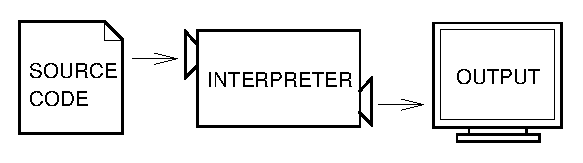
\includegraphics[height=0.77in]{figs/interpret.eps}}
\afterfig

\index{源码}
\index{目标}
\index{可执行代码}

编译器读取程序,完全转换之。在这种情况下,高级语言程序叫做源码,编译后的程序叫做目标代码或者叫可执行代码。一旦程序被编译,就可以直接执行,无须再编译。

\beforefig
\centerline{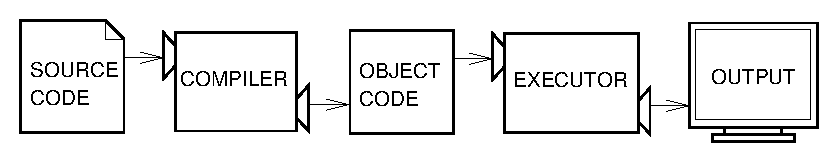
\includegraphics[height=0.77in]{figs/compile.eps}}
\afterfig

一般地,我们把python当作是解释型语言,因为用Python编写的程序是通过
解释器执行的。有两种使用解释器的方式:交互模式和脚本模式。在交互模式
下,你可以输入Python程序,然后解释器输出结果:

\index{交互模式}
\index{脚本模式}

\beforeverb
\begin{verbatim}    
>>>1 + 1
2
\end{verbatim} %直接输出以上两句,包括空白和断行
\afterverb

锯齿符,{\tt >>>},是提示符,解释器用它来表明自己已经准备好了,
如果你输入{\tt 1 + 1},解释器显示{\tt 2}。\\

\index{提示符}

另外地,我们可以把代码存储在一个文件里,使用解释器执行文件,此时这个
文件被称作脚本。习惯上,Python脚本的扩展名为{\tt .py}。

\index{脚本}

如果要执行Python脚本,我们必须提供给解释器脚本的文件名。在UNIX命令窗口,可以输入{\tt python dinsdale.py}。在其他开发环境中,会有些细节方面的差别。可以在Python官网上(\url{python.org})找到相应的指导。

\index{测试!交互模式}

在交互模式下工作很容易测试一小段代码,因为可以随时输入,并且立刻执行。但如果代码量较大,我们必须把代码存放在脚本里,这样方便我们以后修改执行。 

\section{什么是程序}

程序就是指令集合,这些指令说明了如何执行计算。计算可能是数学上的,例如解决等式组或者计算多项式的平方根。但是也可以是符号计算,比如搜索替换文件的文本或者(非常奇怪)编译一个程序。

\index{程序}

不同的语言有一些细节上的差异。但是他们有一些共有的指令:

\begin{description}

\item[输入:] 从键盘获取数据,文件,或者从其他设备。

\item[输出:] 在显示器上显示数据或者把数据输出到文件或其他设备。

\item[数学运算:] 做基本的数学操作像加法和乘法。

\item[条件执行:]检查条件,然后执行正确的语句。

\item[循环:]重复执行一些动作,通常有些变化。

\end{description}

信不信由你,就是这样。我们用过的任何一个软件,无论多么复杂,基本上都是由与这些相似的指令组成。所以,我们可以这么理解:编程就是把复杂庞大的任务分解为一系列的小任务,知道这些小任务简单到可以用这些基本的指令表示。

\index{算法}

这个有点模糊,但是当我们讲到算法的时候,我们再回过头来聊这个话题。

\section{什么是调试?}
\index{调试}
\index{臭虫}

有三种错误经常在程序中出现:语法错误,运行时错误和语义错误。为了能够快速的跟踪捕捉到他们,区分他们之间的诧异还是很有好处的。

\subsection{语法错误}
\index{语法错误}
\index{错误!语法}
\index{错误信息}

Python只能执行语法正确的程序;否则,解释器就会报错。语法指的是程序的结构和结构的规则。\index{syntax 语法}
比如,括号必须是成对出现,所以{\tt (1 + 2)}是合法的,但{\tt 8)}就是语法错误。

\index{parentheses!matching  括号!匹配}
\index{syntax 语法}
\index{cummings, e. e. 康明思}

在英语中,读者可以忍受大多数语法错误,这就是为什么我们玩味E. E康明思的诗歌,而没有提出任何错误信息的原因。Python不会这么仁慈。如果在你程序的某个地方出现了哪怕是一个语法错误,Python也会显示错误信息然后退出,你也不能再继续执行程序。在你初学编程的几周里,你很可能会花费大量的时间追踪,捕捉语法错误。一旦你有经验了,你犯的错误就更少,并且也能很快的发现他们。

\subsection{运行时错误}
\label{runtime 运行时}
\index{runtime error 运行时错误}
\index{error!runtime 错误!运行时}
\index{exception 异常}
\index{safe language 安全语言}
\index{language!safe 语言!安全}


第二中错误是运行时错误,之所以这么命名是因为从这种错误知道程序开始运行才会出现。这些错误也叫做异常,因为他们通常表明异常的事情发生了。\\

运行时错误在前几章的简短的代码中比较少见,因此你可能会有一段时间才会遇到。

\section{语义错误}
\index{semantics 语义}
\index{semantics errors 语义错误}
\index{error!semantic 错误!语义}
\index{error message 错误信息}

第三中错误是语义错误。如果有语义错误,程序会成功运行(即计算机不会产生任何的错误信息),但是它却没有做对!计算机做了另外的事。确切的说,计算机确实做了你告诉他的指令。

\subsection{试验性的调试}

你必须拥有的一条技能是调试。尽管在这个过程中,你可能很受伤,但,调试是编程中最具有挑战,最有意思,最能考验智力的一部分。\\

\index{experimental debugging 实验性的调试}
\index{debugging!experimental 调试!实验}

某种程度上,调试就像是侦探。你面对着很多线索,必须推断导致你看到的结果的过程和事件。\\

调试也像是一个科学实验。一旦你意识到错误的地方,改正她,再尝试。如果你的假想是正确的,你就可以预测出改变带来的结果,你也就离能够执行的程序更近一步了。如果你的猜想是错误的,你不得不提出一个新的。正如Sherlock Holmoes指出的,“当你移除了不可能的,留下来的无论是什么,也不论多么不可能,都是真理。(A. Conan Doyle, {\em The Sign of Four})\\

\index{Holems, Sherlock}
\index{Doyle, Arthur Conan}

对某些人来说,编程和调试是同时完成的。也就是,编程是不断调试,直到看到想要结果的过程。理念就是:你必须以一个能够工作的程序开始,然后做些小改动,随着进度不断调试他们,这样就总是有一个可工作的程序。\\

比如:Linux是一个包含成千上万行代码的操作系统,但它也是从一个Linux Torvalds用来研究Intel 80386芯片的小程序开始的。按照Larry Greenfield的说法,“Linus的早期项目就是一个在打印AAAA和BBBB之间切换的程序。“({\em The Linux Users' Guide} Beta Version 1)。

\index{Linux}

接下来的章节将介绍更多的调试建议还有其他的编程经验。

\section{正式语言和自然语言}
\index{formal language 正式语言}
\index{natural language 自然语言}
\index{language!formal 语言!正式}
\index{language!natural 语言!自然}

自然语言是人们日常说的语言,比如英语,西班牙语和法语。他们不是人民设计的(尽管人们努力的强加一些规则);他们是自然发展的。\\

正式语言是人们为了特别的应用而设计的语言。比如,数学家使用的符号就是一门正式语言,它很擅长揭示数字和符号之间的联系。化学家用正式语言代表分子的化学结构。最重要的是:

\begin{quote}
{编程语言是正式语言,是被设计来表达计算的。}
\end{quote}

正式语言倾向于有严谨的语法规则。比如,$3 + 3 = 6$是语法争取的数学语句。但是$3 += 3 \mbox{\$} 6$ 不是。$H_2O$是语法正确的化学分子式,但$_2Zz$ 不是。\\

语法规则涉及到两个方面:标记和结构。标记是语言的最基本元素,比如字,数字和化学元素。$3 += 3 \mbox{\$} 6$的一个问题是$\$$不是一个合法的数学标记(至少据我所知)。相似的,$_2Zz$不合法是因为没有元素的缩写是$Zz$。

\index{token 标记}
\index{structure 结构}

第二种语法错误涉及到语句的结构,也就是,标记被安排的方式。语句$3 + = 3 \mbox{\$} 6$是非法的因为尽管$+$和$=$是合法的标记,但我们不能把两个相连。同样的,在化学分子式中,下标必须在元素之后,不是前面。

\begin{ex}
写一个结构正确的英语句子,同时标记也必须合法。然后写一个结构不合理但是标记合法的句子。
\end{ex}

当阅读一个英文句子或者正式语言的一个语句,必须明确句子的结构(尽管对于自然语言来说,这个是潜意识的)。这个过程叫做句法分析。

\index{parse 句法分析}

比如,当你听到一个句子,“一便士硬币掉了”,你理解“一便士硬币”是主语,“掉了”是谓语。一旦你分析了这个句子,你就明确句子的意思。假如你知道一个便士是什么,并且什么是掉了,你就会明白这个句子的一般含意。\\

尽管正式语言和自然语言有很多共同点---标记,结构,语法和语义---也存在一些不同点:

\index{ambiguity 二义性}
\index{redundancy 冗余性}
\index{literalness 无修饰性}

\begin{description}

\item[二义性:]自然语言充满了二义性(模糊性),人们利用上下文来区分。正式语言被设计成近乎没有二义性,这也意味着每个语句都有明确的意思,无论上下文。

\item[冗余性:]为了弥补二义性和减少误解,自然语言设置了很多冗余。因此自然语言是冗长的。自然语言更简短,精确。

\item[无修饰性:]自然语言充满了习语和隐喻。如果我说“一便士硬币掉了”,也许根本没有便士也没有东西掉了\footnote{这个习语意思是某人困惑之后恍然大悟。}。正式语言表达了是精确的意思。

\end{description}

成长过程中,说自然语言的人---每个人---通常在调整自己适应正式语言的过程中都会经历痛苦。某种程度上,正式语言和自然语言之间的区别就像诗歌和散文\footnote{译者:这里的散文不是诗化的散文,像余光中老前辈开启的诗化散文}之间的区别,甚至更多:

\index{poetry 诗歌}
\index{prose 散文}

\begin{description}

\item[诗歌:]单词的运用既是为了语义的需要,也是为了音韵的需要,整首诗创造了一种情感共鸣。二义性不仅很常见,而且常常是故意安排的。

\item[散文:]单词的字面意思更加重要,结构也表达了更多的意思。散文比诗歌更容易分析,但是仍然具有二义性。

\item[程序:]计算机程序是无二义性。可以通过分析标记和结构完全理解。


\end{description}

这里给些读程序时候的一些建议(包括其他正式语言).第一,记住正式语言是比自然语言要晦涩的,所以要花长时间阅读。其次,结构也是非常重要的,所以,从头到位,从左到右阅读通常不是一个好的办法,可以学习在大脑中分析程序,识别标记的意思,然后解释结构。最后,细节也很重要。一些拼写和标点上细小的错误(在自然语言中可以忽略的),有时会在正式语言中掀起大浪。

\section{第一个程序}
\label{hello}
\index{Hello, World}

通常,学习新语言的第一个程序就是"hello world", 应为所做的就是显示单词,"Hello , World!".在Python中,看起来是:

\beforeverb
\begin{verbatim}
print 'Hello, World!'
\end{verbatim}
\afterverb

这是一个print语句的例子\footnote{在Python3.0中,{\tt print}是一个函数,不是一个语句了,所以语法是{\tt print("Hello, World!")}。我们不久就要接触到函数了!  译注:在本书翻译时python 2.7 和python3.1已经发布,python 3.2的release 版也即将发布},没有真正在纸上打印东西。它在显示器上显示了一个值。在这种情况下,结果是单词

\index{Python 3.0}

\beforeverb
\begin{verbatim}
Hello, World!
\end{verbatim}
\afterverb

程序中的引号标志了要被显示的文本的开始和结束,他们不会出现在结果中。

\index{quotation mark 引号}
\index{print statement print 语句}
\index{statement!print 语句!打印}

一些人通过"Hello, World!"程序的简洁程度来判断编程语言的好坏。按照这个标准,Python确实非常好!


\section{调试}
\index{debugging 调试}

坐在电脑前面看这本书是个不错的方法,你可以随时尝试书中的例子。你可以在
交互模式下运行大多数的程序,但是如果你把代码放在一个脚本里,也是很容易尝试改变一些内容的。\footnote{译者注:我的理解是,可以很方便的
改动某些变量或者语句,然后执行}\\

无论何时,尝试一个新的特点的时候,你应该故意的犯些错误。比如,在"Hello, World!"程序中,如果忽略了双引号其中之一,会发生什么?如果把两个引号都忽略了,又会怎样?如果拼错了{\tt print}了呢?\\

\index{error message 错误信息}

这种实验能够有效的帮助你记住你看的内容,同时也对调试有好处,因为你知道了错误信息的意思了。现在故意的犯错误总比以后猝不及防的犯错误要好的多。\\

编程,特别是调试,有时带来很强的情绪。你在一个困难的bug里苦苦挣扎,你可能变得怒不可遏,苦恼不堪,甚至羞愧不已。\\

有证据表明,人们很容易把电脑当成人来对待\footnote{参看Reeves和Nass,{\it The Media Equation:How People Treat Computers, Television, and New Media Like Real People and Places}.}.当电脑工作正常,我们把它们当作是队友,当电脑不给力时,我们把它们当成粗鲁顽固的人。\\

\index{debugging!emotional response 调试!情绪反应}
\index{emotional debugging 情绪调试}

为这些反应作准备也许会帮助你合理的处理。一个方法是把电脑当作一个员工,他既拥有一定力量,比如速度和精度,也会有特别的缺点,比如缺少默契,没有能力理解大的图片。\\

你的工作就是做一个好的经理:发掘有效的方法扬长补短。并且寻找方法利用你的情绪来投入到解决问题中,不要让你的(不良)反应干扰你工作的能力.\\

学习调试是令人沮丧的,但是一种宝贵的技巧,在编程的其他领域也是大有裨益的。在每章的末尾,都有一个调试段落,像这个一样,是我调试经验的总结。我希望他们对你有益!

\section{术语表}
\begin{description}

\item[problem solving 问题解决:]表述问题,发现解,表达解的过程。

\item[high-level language 高级语言:]像Python一样的程序设计语言,被设计让人们易读易写程序。

\item[low-level language 低级语言:]设计让计算机容易执行的程序设计语言;也叫做“机器语言”或者“汇编语言”。

\item[portability 可移植性:]程序可以在一台或多台电脑执行的属性。

\item[interpret 解释:]逐行逐行解释执行用高级语言编写的程序。

\item[compile 编译:]把用高级语言编写的程序转换成低级语言。
\index{compile 编译}

\item[source code 源码:]未编译的高级语言编写的程序。

\item[object code 目标代码:] 编译器转换程序后的输出。
\index{object code 目标代码}

\item[executable 可执行代码:] 目标代码的别名,可以被执行。
\item{executable 可执行代码}
\item[prompt 提示符:] 解释器显示的字符,表明做好准备让用户输入。
\index{prompt 提示符}

\item[script 脚本:]存储在文件中的程序。
\index{script 脚本}

\item[interactive mode 交互模式:] 一种通过输入命令和表达式的使用python解释器的方式。
\index{interactive mode 交互模式}

\item[script mode 脚本模式:] 一种使用Python解释器的方式,Python解释器读取脚本中的语句执行。
\index{script mode 脚本模式}

\item[program 程序:]指明计算的指令集合。
\index{program 程序}


\item[algorithm 算法] 求解一类问题的通用过程。
\index{algorithm}

\item[bug:] 程序的错误。
\index{bug}

\item[debugging 调试:]发现,去除程序错误的过程。
\index{debugging 调试}

\item[syntax 语法] 程序的结构。
\index{syntax 语法} 

\item[syntax error 语法错误:]使程序不能正确解析的错误。
\index{syntax error}


\item[exception 异常:]程序在运行时发现的错误。
\index{exception 异常}

\item[semantics  语义:]程序的含意。
\index{semantics 语义}

\item[semantics error 语义错误:] 程序中的错误,使计算机执行另外的程序。
\index{semantics error 语义错误}

\item[natural language 自然语言:]人们日常交流用的语言,自然发展的。
\index{natural language 自然语言}

\item[formal language 正式语言:]人民为了某种特殊目的设计的语言,比如,代表数学思想或者计算机程序,所有的程序设计语言都是正式语言。
\index{formal language 正式语言}

\item[token 标记:]程序语法结构的最基本元素,类似于自然语言的单词。
\index{token 标记}

\item[parse 句法分析:]检查程序,分析语法结构。
\index{parse 句法分析}

\item[print statement print 语句:]一条指示Python解释器显示一个值的指令。
\index{print statement print 语句}

\index{statement!print 语句!打印}

\end{description}

\section{练习}

\begin{ex}
打开浏览器浏览Python官网\url{python.org}.这个页面包含了Python的一些信息,还有和Python相关的连接。你可以查看Python官方文档。\\

比如,在搜索框里输入{\tt print},第一个链接就是{\tt print}语句的文档。此时,并不是所有的信息对你都有意义,但是知道它们在哪里总是有好处的。

\index{documentation 文档}
\index{python.org}
\end{ex}

\begin{ex}
启动Python的解释器,输入{\tt help()}启动在线帮助工具。或者你也可以输入\verb"help('print')" 获得关于{\tt print}语句的信息。\\

如果没有成功,你或许需要安装额外的Python官方文档,或者设置环境变量。这个依赖于你使用的操作系统和Python解释器版本。

\index{help utility 帮助工具}
\end{ex}


\begin{ex}
打开Python解释器,我们暂且把它作为计算器。关于数学操作的语法,Python和标准的数学符号很相似。比如,符号{\tt +},{\tt -} 和{\tt /}表示加减,除。乘法的符号是{\tt *}。\\

如果43分钟30秒,跑了10公里,每英里花费的时间是多少?你的平均速度是多少英里每小时?(Hint:一英里等于1.61公里)。

\index{caculator 计算器}
\index{running pace 跑步速度}
\end{ex}
























